\documentclass{beamer}
\usepackage[italian]{babel}
\usepackage[utf8]{inputenc}
\usepackage[T1]{fontenc}

% Personal commands
\newcommand{\code}[1]{\mbox{\texttt{#1}}}
\newcommand{\command}[1]{\mbox{\texttt{#1}}}
\newcommand{\file}[1]{\mbox{\texttt{#1}}}

% Beamer options
\beamertemplatenavigationsymbolsempty
\setbeamertemplate{bibliography item}{}
\setbeamertemplate{caption}{\insertcaption}
\setbeamertemplate{footline}[frame number]

\title{Introduzione alla cyber security, ethical hacking e CTF}
\author[leot]{Leonardo Taccari \\ {\footnotesize \texttt{<s1069964@studenti.univpm.it>}}}
\date{}

\begin{document}

% Title of the presentation
\begin{frame}
\maketitle
\end{frame}

% Outline
\begin{frame}{Sommario}
\tableofcontents
\end{frame}

\section*{Un'occhiata a notizie recenti riguardante la cyber security}
\begin{frame}{\insertsection}
\begin{itemize}
\item Perché la cyber security è importante?
\item Proviamo a "sfogliare" i giornali delle ultime settimane
\item Come questi incidenti possono coinvolgerci?
\end{itemize}
\end{frame}

\subsection*{Ragazzo viola registro elettronico per cambiare i suoi voti}
\begin{frame}{\insertsection}{\insertsubsection}
\begin{figure}
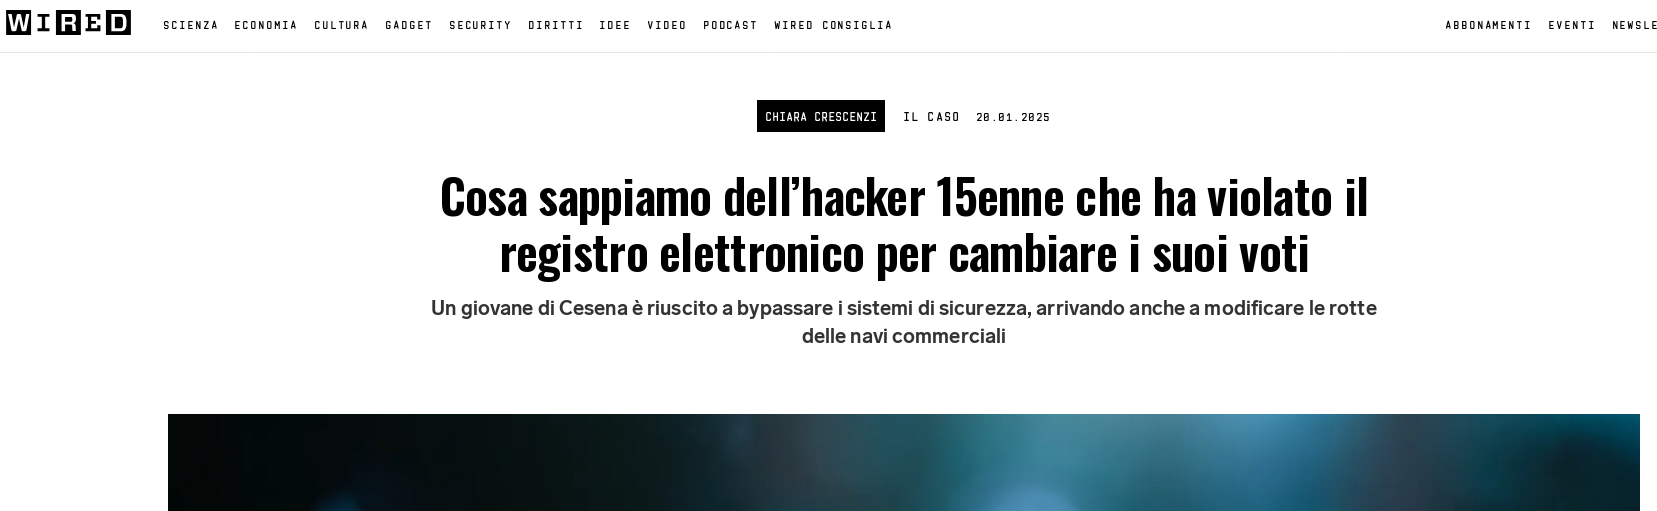
\includegraphics[width=0.95\textwidth]{imgs/news-wired-hacker-15enne.png}
\caption{Cosa sappiamo dell'hacker 15enne che ha violato il registro elettronico
per cambiare i suoi voti, Chiara Crescenzi, Wired, 20/01/2025
\href{https://www.wired.it/article/hacker-15enne-voti-scolastici/}{(link)}}
\end{figure}
\end{frame}

\subsection*{Rubati dati personali di più di 5.5 milioni di utenti InfoCert}
\begin{frame}{\insertsection}{\insertsubsection}
\begin{figure}
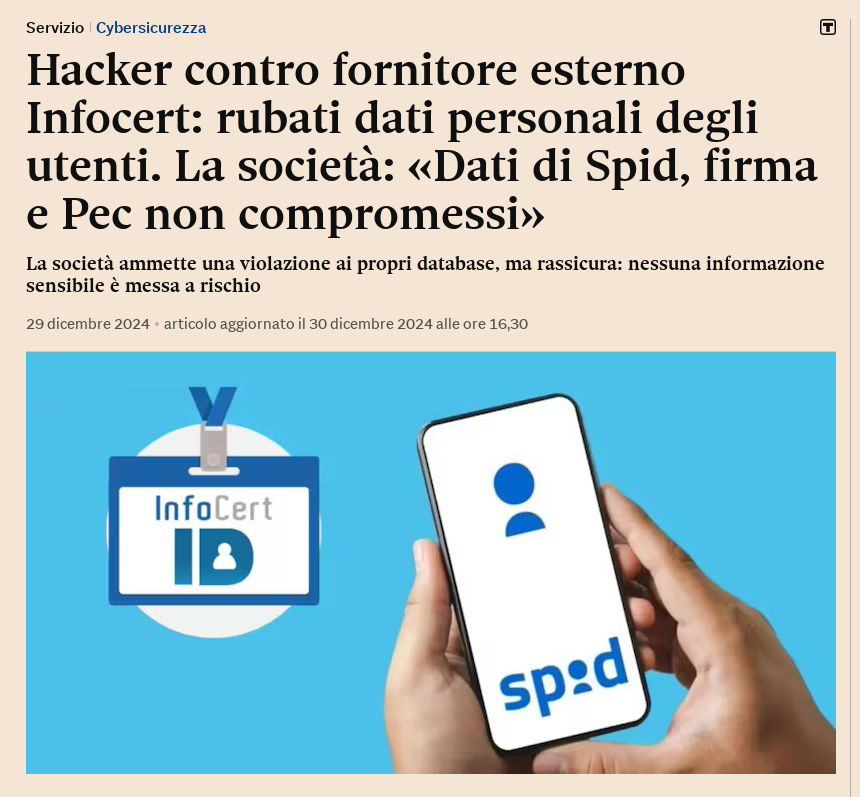
\includegraphics[width=0.6\textwidth]{imgs/news-ilsole24ore-infocert.png}
\caption{Hacker contro fornitore esterno Infocert: rubati dati personali degli
utenti. La società: «Dati di Spid, firma e Pec non compromessi», Il Sole 24 Ore,
29/12/2024
\href{https://www.ilsole24ore.com/art/spid-hacker-contro-infocert-rubate-informazioni-milioni-utenti-AGnDOQ2B}{(link)}}
\end{figure}
\end{frame}

\subsection*{Fuga di dati da Volkswagen: accessibili in chiaro posizioni geografiche e dati personali dei possessori di 800000 automobili}
\begin{frame}{\insertsection}{\insertsubsection}
\begin{figure}
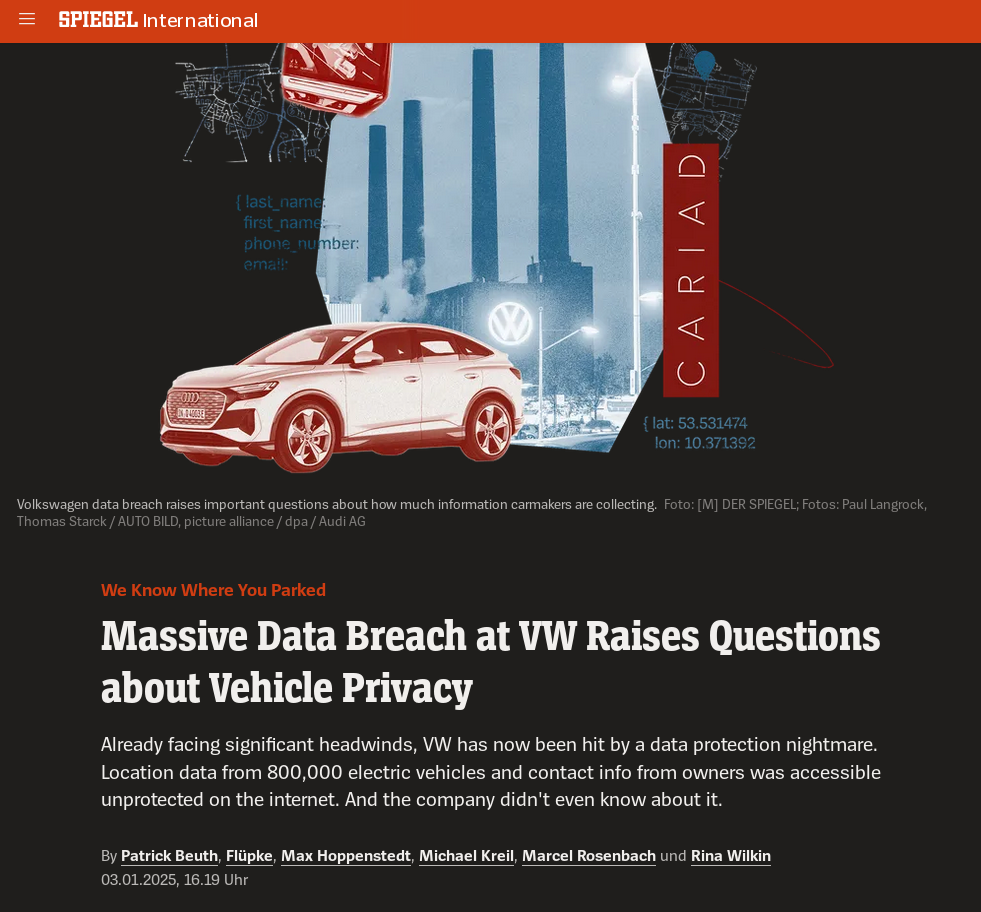
\includegraphics[width=0.55\textwidth]{imgs/news-spiegel-vw-dataleak.png}
\caption{Massive Data Breach at VW Raises Questions about Vehicle Privacy,
Patrick Beuth, Flüpke, Max Hoppenstedt, Michael Kreil, Marcel Rosenbach e Rina
Wilkin, Der Spiegel, 03/01/2025
\href{https://www.spiegel.de/international/business/we-know-where-you-parked-massive-data-breach-at-vw-raises-questions-about-vehicle-privacy-a-4b1cb926-2edb-42ea-92fb-5000cd378fc5}{(link)}}
\end{figure}
\end{frame}

\section{Concetti fondamentali}
\begin{frame}{\insertsection}
\end{frame}

\subsection{Cyber Security}
\begin{frame}{\insertsubsection: definizioni}
Alcune definizioni dal NIST~\footnote{National Institute of Standards
and Technology} Computer Security Resource Center (CSRC) Glossary (via
NIST SP 800-30).
\end{frame}

\subsubsection*{Cyberspace}
\begin{frame}{\insertsubsection: definizioni}{\insertsubsubsection}
\begin{block}{\insertsubsubsection}
A global domain within the information environment consisting of the
interdependent network of information systems infrastructures including
the Internet, telecommunications networks, computer systems, and
embedded processors and controllers.
\end{block}
\end{frame}

\subsubsection*{Cyber Attack}
\begin{frame}{\insertsubsection: definizioni}{\insertsubsubsection}
\begin{block}{\insertsubsubsection}
An \alert{attack}, via \alert{cyberspace}, targeting an enterprise's
use of cyberspace for the purpose of disrupting, disabling, destroying,
or maliciously controlling a computing environment/infrastructure; or
destroying the integrity of the data or stealing controlled
information.
\end{block}
\end{frame}

\subsubsection*{Cyber Security}
\begin{frame}{\insertsubsection: definizioni}{\insertsubsubsection}
\begin{block}{\insertsubsubsection}
The ability to protect or defend the use of \alert{cyberspace} from
\alert{cyber attacks}.
\end{block}
\end{frame}

\subsection{CIA: Confidentiality, Integrity, Availability}
\begin{frame}{\insertsubsection}
I pilastri della \alert{cyber security} sono costituiti dalla "triade" \alert{CIA}:
\alert{Confidentiality}, \alert{Integrity}, \alert{Availability}.
\end{frame}

\subsubsection*{Confidentiality (Confidenzialità, Riservatezza)}
\begin{frame}{\insertsubsection}{\insertsubsubsection}
\begin{block}{\insertsubsubsection}
La \alert{confidentiality} (confidenzialità, riservatezza) è la
proprietà che garantisce che le risorse sono accessibili solo ai
soggetti autorizzati.
\end{block}
\end{frame}

\subsubsection*{Integrity (Integrità)}
\begin{frame}{\insertsubsection}{\insertsubsubsection}
\begin{block}{\insertsubsubsection}
La \alert{integrity} (integrità) è la proprietà che garantisce che le
risorse non siano alterate o distrutte da soggetti non autorizzati ad
accederle.
\end{block}
\end{frame}

\subsubsection*{Availability (Disponibilità)}
\begin{frame}{\insertsubsection}{\insertsubsubsection}
\begin{block}{\insertsubsubsection}
La \alert{availability} (disponibilità) è la proprietà che garantisce un accesso
affidabile e tempestivo alle risorse da parte dei soggetti autorizzati.
\end{block}
\end{frame}

\subsubsection*{Cyber security e CIA (Confidentiality, Integrity, Availability)}
\begin{frame}{\insertsubsection}{\insertsubsubsection}
\begin{block}{\insertsubsubsection}
Quando una o più di queste proprietà viene violata si ha un problema di
\alert{cybersecurity}.
\end{block}
\end{frame}

\subsubsection*{Vulnerabilità}
\begin{frame}{\insertsubsection}{\insertsubsubsection}
\begin{block}{\insertsubsubsection}
Bug, difetto, debolezza o esposizione accidentale di un'applicazione, sistema,
dispositivo o servizio che può portare alla violazione di
\alert{confidentiality}, \alert{integrity} o \alert{availability}.
\end{block}
\end{frame}

\subsubsection*{Esempio: Registro elettronico}
\begin{frame}[allowframebreaks]{\insertsubsection}{\insertsubsubsection}
Le proprietà CIA dipendono dal sistema considerato. Cerchiamo di
contestualizzarle nel Registro elettronico!
\begin{description}
\item[confidentiality] uno studente può visualizzare solo i propri voti \\
(se uno studente potesse vedere i voti di altri studenti si avrebbe una
\alert{fuga di informazioni} (\alert{unauthorized disclosure}))
\item[integrity] uno studente può accedere ai voti solo in lettura, non
può modificarli; un docente può assegnare una votazione che va da 1 a 10 \\
(se uno studente potesse modificare i voti o un docente potesse mettere una
votazione di 11 si avrebbe una \alert{modifica non autorizzata}
(\alert{unauthorized modification}) o \alert{modifica impropria}
(\alert{improper modification}))
\item[availability] uno studente deve poter leggere i voti, un docente deve
poter assegnare i voti (se un docente non potesse assegnare delle valutazioni si
avrebbe una \alert{"ritenuta" non autorizzata} (\alert{unauthorized withholding}))
\end{description}
\end{frame}

\subsection{Ethical Hacking}
\begin{frame}{\insertsubsection}
\end{frame}

\subsubsection*{Hacker}
\begin{frame}{\insertsubsection}{\insertsubsubsection}
Da `The Jargon File (version 4.4.7, 29 Dec 2003)':

\begin{block}{\insertsubsubsection}
\alert{hacker} n. [originally, someone who makes furniture with an axe]

1. A person who enjoys exploring the details of programmable
   systems and how to stretch their capabilities, as opposed to most
   users, who prefer to learn only the minimum necessary. RFC1392,
   the Internet Users' Glossary, usefully amplifies this as: «A
   person who delights in having an intimate understanding of the
   internal workings of a system, computers and computer networks in
   particular».
\end{block}
\end{frame}

\begin{frame}{\insertsubsection}{\insertsubsubsection}
Da `Errore di Sistema' di Edward Snowden:

\begin{quotation}
È da qui che ha origine l'attività dell'hacker: dalla consapevolezza del
legame sistematico tra input e output, tra causa ed effetto. L'hacker
non esiste soltanto in informatica, ma ovunque ci siano delle regole.
Per hackerare un sistema occorre conoscere le sue regole ancor meglio di
chi le ha create o di chi quel sistema lo gestisce, e sfruttare al
massimo la discrepanza tra il modo in cui il sistema dovrebbe funzionare
e il suo effettivo funzionamento. Nel trarre vantaggio da questi usi non
intenzionali, gli hacker non infrangono le regole, ma piuttosto le
demistificano.
\end{quotation}
\end{frame}

\subsubsection*{\{Black,Gray,White\} Hacker}
\begin{frame}{\insertsubsection}{\insertsubsubsection}
Da `The Jargon File (version 4.4.7, 29 Dec 2003)':

\begin{block}{\insertsubsubsection}
\alert{black hat}

1. [common among security specialists] A \alert{cracker}, someone bent on
   breaking into the system you are protecting. Oppose the less common
   \alert{white hat} for an ally or friendly security specialist; the term
   \alert{gray hat} is in occasional use for people with cracker skills operating
   within the law, e.g. in doing security evaluations. All three terms
   derive from the dress code of formulaic Westerns, in which bad guys
   wore black hats and good guys white ones.
\end{block}
\end{frame}

\subsubsection*{Ethical hacker}
\begin{frame}[allowframebreaks]{\insertsubsection}{\insertsubsubsection}
Un \alert{ethical hacker} è un \alert{white hat hacker} e opera legalmente ed in
modo etico.

\begin{alertblock}{Legge 547 del 1993, Art.615-ter. (Accesso abusivo ad
un sistema informatico e telematico).}
\begin{quote}
Chiunque abusivamente si introduce in un sistema informatico o
telematico protetto da misure di sicurezza ovvero vi si mantiene contro
la volontà espressa o tacita di chi ha il diritto di escluderlo, è
punito con la reclusione fino a tre anni.
\end{quote}
\end{alertblock}

In altre parole, possiamo esclusivamente - legalmente - attaccare sistemi
di cui abbiamo un permesso. Possibili modi per fare ciò:

\begin{description}
\item[Bug Bounty] programmi in cui organizzazioni permettono a ricercatori di
trovare vulnerabilità offrendo loro una ricompensa (esempi:
\href{https://www.hackerone.com/}{HackerOne},
\href{https://www.intigriti.com/}{Intigriti},
\href{https://www.bugcrowd.com/}{Bugcrowd})
\item[CTF (Capture the Flag)] competizioni di cyber security (le vedremo tra
poco più in dettaglio!)
\end{description}
\end{frame}

\subsection{Software Libero}
\begin{frame}{\insertsubsection}
\end{frame}

\section{Capture The Flag (CTF)}
\begin{frame}{\insertsection}
\end{frame}

\section{Conclusioni}
\begin{frame}{\insertsection}
\end{frame}

\end{document}
